% !TeX root = RJwrapper.tex
\title{Bootstrapping Clustered Data in R using lmeresampler}
\author{by Adam Loy and Jenna Korobova}

\maketitle

\abstract{%
Linear mixed-effects models are commonly used to analyze clustered data structures. There are numerous packages to fit these models in R and conduct likelihood-based inference. The implementation of resampling-based procedures for inference are more limited. In this paper, we introduce the \pkg{lmeresampler} package for bootstrapping nested linear mixed-effects models fit via \pkg{lme4} or \pkg{nlme}. Bootstrap estimation allows for bias correction, adjusted standard errors and confidence intervals for small samples sizes and when distributional assumptions break down. We will also illustrate how bootstrap resampling can be used to diagnose this model class. In addition, \pkg{lmeresampler} makes it easy to construct interval estimates of functions of model parameters.
}

\hypertarget{introduction}{%
\subsection{Introduction}\label{introduction}}

Clustered data structures occur in a wide range of studies. For example, students are organized within classrooms, schools, and districts, imposing a correlation structure that must be accounted for in the modeling process. Similarly, cholesterol measurements could be tracked across time for a number of subjects, resulting in measurements being grouped by subject. Other names for clustered data structures include grouped, nested, multilevel, hierarchical, longitudinal, repeated measurements, and blocked data. The covariance structure imposed by clustered data is commonly modeled using linear mixed-effects (LME) models, also referred to as hierarchical linear or multilevel linear models (J. C. Pinheiro and Bates 2000; Raudenbush and Bryk 2002; Goldstein 2011).

In this paper, we restrict attention to the Gaussian response LME model for clustered data structures. For cluster
\(i=1, \ldots, g\), this model is expressed as
\begin{equation}
    \underset{(n_i \times 1)}{\boldsymbol{y}_i} = \underset{(n_i \times p)}{\boldsymbol{X}_i} \ \underset{(p \times 1)}{\boldsymbol{\beta}} + \underset{(n_i \times q)}{\boldsymbol{Z}_i} \ \underset{(q \times 1)}{\boldsymbol{b}_i} + \underset{(n_i \times 1)}{\boldsymbol{\varepsilon}_i},
    \label{eq:lme}
\end{equation}
where
\begin{equation}
\boldsymbol{\varepsilon}_i \sim \mathcal{N}(\boldsymbol{0}, \sigma^2 \boldsymbol{I}_{n_i}),   \boldsymbol{b}_i \sim \mathcal{N}(\boldsymbol{0}, \boldsymbol{D}),
\label{eq:dsns}
\end{equation}
where \(\boldsymbol{\varepsilon}_i\) and \(\boldsymbol{b}_i\) are independent for all \(i\), \(\boldsymbol{\varepsilon}_i\) is independent of \(\boldsymbol{\varepsilon}_j\) for \(i\ne j\), and \(\boldsymbol{b}_i\) is independent of \(\boldsymbol{b}_j\) for \(i\ne j\). Here, \(\boldsymbol{0}\) denotes a vector of zeros of length \(n_i\) (the number of observations in group \(i\)), \(\boldsymbol{I}_{n_i}\) denotes the \(n_i\)-dimensional identity matrix,
and \(\boldsymbol{D}\) is a \(q \times q\) covariance matrix.

In R, the two most popular packages to fit LME models are \CRANpkg{nlme} (J. Pinheiro et al. 2017) and \CRANpkg{lme4} (Bates et al. 2015). Both packages fit LME models using either maximum likelihood or restricted maximum likelihood methods. These methods rely on the distributional assumptions placed on the residual quantities, \(\boldsymbol{\varepsilon}_i\) and \(\boldsymbol{b}_i\), as well as large enough sample sizes. While some aspects of LME models are quite robust to model misspecification, others are more sensitive, leading to biased estimates and/or incorrect standard errors. Jacqmin-Gadda et al. (2007) found that inference for the fixed effects is robust if the distribution of the error terms, \(\boldsymbol{\varepsilon}_i\), is non-normal or heteroscedastic, but that variance components and random effects are biased if the covariance structure for the error terms is misspecified. The fixed intercept is not robust to misspecification of the random effects (Hui, Müller, and Welsh 2021). In addition, misspecification of the random effects distribution can lead to biased estimates of the variance components and undercoverage of the confidence intervals (Hui, Müller, and Welsh 2021). In cases where distributional assumptions are suspect, bootstrapping provides an alternative inferential approach that leads to consistent, bias-corrected parameter estimates, standard errors, and confidence intervals. Standard errors and confidence intervals for functions of model parameters are also easily calculated using a bootstrap procedure, and are available even in situations where closed-form solutions are not.

A variety of bootstrap procedures for clustered data and the LME model have been proposed and investigated, including the cases (non-parametric) bootstrap, the residual bootstrap, the parametric bootstrap, the random effect block (REB) bootstrap, and the wild bootstrap (Morris 2002; Carpenter, Goldstein, and Rasbash 2003; Field and Welsh 2007; Chambers and Chandra 2013; Modugno and Giannerini 2015). Van der Leeden, Meijer, and Busing (2008) provide a thorough overview of bootstrapping LME models. Sánchez-Espigares and Ocaña (2009) developed a full-featured bootstrapping framework for LME models in R; however, this package is not available and there appears to be no active development. Consequently, R users must pick and choose packages based on what bootstrap procedure they wish to implement. The parametric bootstrap is available in \pkg{lme4} via the \texttt{bootMer()} function, as is the semi-parametric (residual) bootstrap proposed by Morris (2002). The \texttt{simulateY()} function in \pkg{nlmeU} (Galecki and Burzykowski 2013) makes it easy to simulate values of the response variable for \texttt{lme} model objects; however, the user is required to implement the remainder of the parametric bootstrap. Chambers and Chandra (2013) made R code available to implement their REB bootstrap as well as the parametric bootstrap and the residual bootstrap proposed by Carpenter, Goldstein, and Rasbash (2003) for LME models fix via \texttt{nlme::lme()}. Unfortunately, these functions were not published on CRAN or extended to models fit via \texttt{lme4::lmer()}. Bootstrap procedures for specific inferential tasks have also been implemented. The parametric bootstrap has been implemented to carry out likelihood ratio tests for the presence of variance components in \CRANpkg{RLRsim} (Scheipl, Greven, and Kuechenhoff 2008). \CRANpkg{pbkrtest} (Halekoh and Højsgaard 2014) provides a Kenward-Roger approximation for performing F-tests using a parametric bootstrap approach for LME models and generalized LME models. \CRANpkg{rptR} uses the parametric bootstrap to estimate repeatabilities for LME models (Stoffel, Nakagawa, and Schielzeth 2017). Finally, constrained inference for LMEs using the residual bootstrap is implemented in \CRANpkg{CLME} (Farnan, Ivanova, and Peddada 2014).

In this paper, we introduce the \CRANpkg{lmeresampler} package which implements a suite of bootstrap methods for LME models fit using either \pkg{nlme} or \pkg{lme4} in a single package. \pkg{lmeresampler} provides a unified \texttt{bootstrap()} command to reduce cognitive load on the user and also provides access to procedures that were not previously available on CRAN. In the next section, we will clarify some notation and terminology for LME models. In \protect\hyperlink{bootstrap-procedures-for-clustered-data}{Bootstrap procedures for clustered data}, we provide an overview of the bootstrap methods implemented in \pkg{lmeresampler}. We then give an \protect\hyperlink{overview-of-lmeresampler}{Overview of lmeresampler}, discuss a variety of \protect\hyperlink{example-applications}{Example applications} for LME models, and show how to \protect\hyperlink{bootstrapping-in-parallel}{Bootstrapping in parallel} works in \pkg{lmeresampler}. We conclude with a \protect\hyperlink{summary}{Summary} and highlight areas for future development.

\hypertarget{bootstrap-procedures-for-clustered-data}{%
\subsection{Bootstrap procedures for clustered data}\label{bootstrap-procedures-for-clustered-data}}

In \pkg{lmeresampler}, we implement five bootstrap procedures for clustered data: a cases
(i.e., nonparamteric) bootstrap, a residual bootstrap (i.e., semiparametric), a parametric
bootstrap, a wild bootstrap, and a block bootstrap. In this section,
we provide an overview of these bootstrap approaches. Our discussion
focuses on two-level models, but procedures generalize to
higher-level models unless otherwise noted.

\hypertarget{the-cases-bootstrap}{%
\subsubsection{The cases bootstrap}\label{the-cases-bootstrap}}

The cases bootstrap is a fully non-parametric bootstrap that resamples
the clusters in the data set to generate bootstrap
resamples. Depending on the nature of the data, this resampling can be
done only for the top-level cluster, only at the observation-level
within a cluster, or at both levels. The choice of the exact resampling
scheme should be dictated by the way the data were generated, since the
cases bootstrap generates new data by mimicking this process.
Van der Leeden, Meijer, and Busing (2008) provide a cogent explanation of how to select a
resampling scheme. To help ground the idea of resampling, consider a two-level
hierarchical data set where students are organized into schools.

One version of the cases bootstrap is implemented by only
resampling the clusters. This version of the bootstrap is what Field and Welsh (2007) term the
cluster bootstrap and Goldstein (2011) term the non-parametric bootstrap. We would choose this resampling scheme, for example, if schools were chosen at random and then all students within each school were observed. In this case, the bootstrap proceeds as follows:

\begin{enumerate}
\def\labelenumi{\arabic{enumi}.}
\tightlist
\item
  Draw a random sample, with replacement, of size \(g\) from the
  clusters.
\item
  For each selected cluster, \(k\), extract all of the cases to form the
  bootstrap sample \(\left(\boldsymbol{y}^*_k, \boldsymbol{X}^*_k, \boldsymbol{Z}^*_k \right)\).
  Since entire clusters are sampled, the total sample size may differ from the that of the original data set.
\item
  Refit the model to the bootstrap sample and extract the parameter
  estimates of interest.
\item
  Repeat steps 1--3 \(B\) times.
\end{enumerate}

\noindent An alternative version of the cases bootstrap only resamples the
observations within clusters, which makes sense in our example
if the schools were fixed and students were randomly sampled within schools.

\begin{enumerate}
\def\labelenumi{\arabic{enumi}.}
\tightlist
\item
  For each cluster \(i=1,\ldots,g\), draw a random sample of the rows for cluster \(i\), with
  replacement, to form the bootstrap sample
  \(\left(\boldsymbol{y}^*_i, \boldsymbol{X}^*_i, \boldsymbol{Z}^*_i \right)\).
\item
  Refit the model to the bootstrap sample and extract the parameter
  estimates of interest.
\item
  Repeat steps 1--2 \(B\) times.
\end{enumerate}

\noindent A third version of the cases bootstrap resamples both clusters and cases
within clusters. This is what Field and Welsh (2007) term the two-state bootstrap.
We would choose this resampling scheme if both schools and
students were sampled during the data collection process.

\noindent All three versions of the case bootstrap are implemented in \pkg{lmeresampler}. We explain how the resampling is specified in our \protect\hyperlink{overview-of-lmeresampler}{Overview of lmeresampler}. Regardless of which version of the cases bootstrap you choose, it requires the weakest conditions: it only requires that the hierarchical structure in the data set is correctly specified.

\hypertarget{the-parametric-bootstrap}{%
\subsubsection{The parametric bootstrap}\label{the-parametric-bootstrap}}

The parametric bootstrap simulates random effects and error terms from the fitted
distributions to form bootstrap resamples. Consequently, it requires the strongest conditions---that is, the parametric bootstrap assumes that the model, as specified by Equations \eqref{eq:lme} and \eqref{eq:dsns}, is correctly specified.

Let \(\widehat{\boldsymbol \beta}\), \(\widehat{\boldsymbol D}\), and \(\widehat{\sigma}^2\) be maximum likelihood or restricted maximum likelihood estimates of the fixed effects and variance components from the fitted model. The parametric bootstrap is then implemented through the following steps:

\begin{enumerate}
\def\labelenumi{\arabic{enumi}.}
\tightlist
\item
  Simulate \(g\) error term vectors, \(\boldsymbol{e}_i^*\), of length \(n_i\) from \(\mathcal{N}\left(\boldsymbol{0},\widehat{\sigma}^2 \boldsymbol{I}_{n_i} \right)\).
\item
  Simulate \(g\) random effects vectors, \(\boldsymbol{b}_i^*\), from \(\mathcal{N}\left(\boldsymbol{0},\widehat{\boldsymbol{D}} \right)\).
\item
  Generate bootstrap responses \(\boldsymbol{y}^*_i = \boldsymbol{X}_i \widehat{\boldsymbol{\beta}} + \boldsymbol{Z}_i \boldsymbol{b}_i^* + \boldsymbol{e}_i^*\).
\item
  Refit the model to the bootstrap responses and extract the parameter estimates of interest.
\item
  Repeat steps 2--4 \(B\) times.
\end{enumerate}

\hypertarget{the-residual-bootstrap}{%
\subsubsection{The residual bootstrap}\label{the-residual-bootstrap}}

The residual bootstrap resamples the residual quantities from the fitted
LME model in order to generate bootstrap resamples.
There are three general types of residuals for LME models (Haslett and Haslett 2007; Singer, Rocha, and Nobre 2017). \dfn{Marginal residuals} correspond to the errors made using the marginal predictions, \(\widehat{\boldsymbol r}_i = \boldsymbol{y_i} - \widehat{\boldsymbol{y}}_i = \boldsymbol{y}_i - \boldsymbol{X}_i \widehat{\boldsymbol{\beta}}\). \dfn{Conditional residuals} correspond to the errors made using predictions conditioned on the clusters, \(\widehat{\boldsymbol{e}}_i = \boldsymbol{y}_i - \widehat{\boldsymbol{y}}_i| \boldsymbol{b}_i = \boldsymbol{y}_i - \boldsymbol{X}_i \widehat{\boldsymbol{\beta}} - \boldsymbol{Z}_i \widehat{\boldsymbol{b}}_i\). The \dfn{predicted random effects} are the last type of residual quantity and are defined as \(\widehat{\boldsymbol{b}}_i = \widehat{\boldsymbol{D}} \boldsymbol{Z}_i^\prime \widehat{\boldsymbol{V}}_i^{-1}\left(\boldsymbol{y}_i - \boldsymbol{X}_i \widehat{\boldsymbol{\beta}} \right)\) where \(\widehat{\boldsymbol{V}}_i = \boldsymbol{Z}_i \widehat{\boldsymbol{D}}\boldsymbol{Z}_i^\prime + \widehat{\sigma}^2 \boldsymbol{I}_{n_i}\).

A naive implementation of the residual bootstrap would draw random samples, with
replacement, from the estimated conditional residuals
and the best linear unbiased predictors (BLUPS);
however, this will consistently underestimate the variability in the
data because the residuals are shrunken toward zero
(Morris 2002; Carpenter, Goldstein, and Rasbash 2003). Carpenter, Goldstein, and Rasbash (2003) solve
this problem by ``reflating'' the residual quantities so that the empirical
covariance matrices match the estimated covariance matrices prior to resampling:

\begin{enumerate}
\def\labelenumi{\arabic{enumi}.}
\item
  Fit the model and calculate the empirical BLUPs, \(\widehat{\boldsymbol{b}}_i\), and the
  predicted conditional residuals, \(\widehat{\boldsymbol{e}}_i\).
\item
  Mean center each residual quantity and reflate the centered
  residuals. Only the process to reflate the predicted random effects is discussed below, but the process is analogous for the conditional residuals.

  \begin{enumerate}
  \def\labelenumii{\roman{enumii}.}
  \tightlist
  \item
    Arrange the random effects into a \(g \times q\) matrix, where each row contains the predicted random effects from a single group. Denote this matrix as \(\widehat{\boldsymbol{U}}\). Define \(\boldsymbol{\widehat{\Gamma}} = \boldsymbol{I}_g \otimes \widehat{\boldsymbol{D}}\), the block diagonal covariance matrix of \(\widehat{\boldsymbol{U}}\).
  \item
    Calculate the empirical covariance matrix as \(\boldsymbol{S} = \widehat{\boldsymbol{U}}^\prime \widehat{\boldsymbol{U}} / g\). We follow the approach of Carpenter, Goldstein, and Rasbash (2003), dividing by the number of groups, \(g\), rather than \(g-1\).
  \item
    Find a transformation of \(\widehat{\boldsymbol{U}}\), \(\widehat{\boldsymbol{U}}^* = \widehat{\boldsymbol{U}} \boldsymbol{A}\), such that \(\widehat{\boldsymbol{U}}^{*\prime} \widehat{\boldsymbol{U}}^* / g = \boldsymbol{\widehat{\Gamma}}\). Specifically, we will find \(\boldsymbol{A}\) such that \(\boldsymbol{A}^\prime \widehat{\boldsymbol{U}}^\prime \widehat{\boldsymbol{U}} \boldsymbol{A} / g = \boldsymbol{A}^\prime \boldsymbol{SA} = \boldsymbol{\widehat{\Gamma}}\). The choice of \(\boldsymbol{A}\) is not unique, so we use the recommendation given by Carpenter, Goldstein, and Rasbash (2003): \(\boldsymbol{A} = \left(\boldsymbol{L}_D \boldsymbol{L}_S^{-1} \right)^\prime\) where \(\boldsymbol{L}_D\) and \(\boldsymbol{L}_S\) are the Cholesky factors of \(\boldsymbol{\widehat{\Gamma}}\) and \(\boldsymbol{S}\), respectively.
  \end{enumerate}
\item
  Draw a random sample, with replacement, from the set \(\lbrace \boldsymbol{u}_i^* \rbrace\) of size \(g\), where \(\boldsymbol{u}_i^*\) is the \(i\)th row of the centered and reflated random effects matrix, \(\widehat{\boldsymbol{U}}^*\).
\item
  Draw \(g\) random samples, with replacement, of sizes \(n_i\) from the set of the centered and reflated conditional residuals, \(\lbrace \boldsymbol{e}_i^* \rbrace\).
\item
  Generate the bootstrap responses, \(\boldsymbol{y}^*_i\), using the fitted model equation: \(\boldsymbol{y}^*_i = \boldsymbol{X}_i \widehat{\boldsymbol{\beta}} + \boldsymbol{Z}_i \widehat{\boldsymbol{u}}^*_i + \boldsymbol{e}_i^*\).
\item
  Refit the model to the bootstrap responses and extract the parameter
  estimates of interest.
\item
  Repeat steps 3--6 B times.
\end{enumerate}

Notice that the residual bootstrap is a \emph{semiparametric} bootstrap, since it depends on the model structure (both the mean function and the covariance structure) but not the distributional conditions (Morris 2002).

\hypertarget{the-random-effects-block-bootstrap}{%
\subsubsection{The random-effects block bootstrap}\label{the-random-effects-block-bootstrap}}

Another semiparametric bootstrap is the random effect block (REB) bootstrap proposed by Chambers and Chandra (2013). The REB bootstrap can be viewed as a version of the residual bootstrap where conditional residuals are resampled from within clusters (i.e., blocks) to allow for weaker assumptions on the covariance structure of the residuals. The residual bootstrap requires that the conditional residuals are independent and identically distributed, whereas the REB bootstrap relaxes this to only require that the covariance structure of the error terms is similar across clusters. In addition, the REB bootstrap utilizes the marginal residuals to calculate non-parametric predicted random effects rather than relying on the model-based empirical best linear unbiased predictors (EBLUPS). Chambers and Chandra (2013) developed three versions of the REB bootstrap, all of which have been implemented in \pkg{lmeresampler}. We refer the reader to Chambers and Chandra (2013) for a discussion of when each should be used. It's important to note that at the time of this writing, that the REB bootstrap has only been explored and implemented for use with two-level models.

\hypertarget{reb0}{%
\paragraph{REB/0}\label{reb0}}

The base algorithm for the REB bootstrap (also known as REB/0) is as follows:

\begin{enumerate}
\def\labelenumi{\arabic{enumi}.}
\tightlist
\item
  Calculate non-parametric residual quantities for the model.

  \begin{enumerate}
  \def\labelenumii{\alph{enumii}.}
  \tightlist
  \item
    Calculate the marginal residuals for each group, \(\widehat{\boldsymbol{r}}_i = \boldsymbol{y}_i - \boldsymbol{X}_i \widehat{\boldsymbol{\beta}}\).
  \item
    Calculate the non-parametric predicted random effects, \(\tilde{\boldsymbol{b}}_i = \left( \boldsymbol{Z}_i^\prime \boldsymbol{Z}_i \right)^{-1} \boldsymbol{Z}^\prime_i \boldsymbol{r}_i\).
  \item
    Calculate the non-parametric conditional residuals using the residuals quantities obtained in the previous two steps, \(\boldsymbol{\tilde{e}}_i = \widehat{\boldsymbol{r}}_i - \boldsymbol{Z}_i \boldsymbol{\tilde{b}}_i\).
  \end{enumerate}
\item
  Take a random sample, with replacement, of size \(g\) from the set \(\lbrace \tilde{\boldsymbol{b}}_i \rbrace\). Denote these resampled random effects as \(\boldsymbol{\tilde{b}}^*_i\).
\item
  Take a random sample, with replacement, of size \(g\) from the cluster ids. For each sampled cluster, draw a random sample, with replacement, of size \(n_i\) from that cluster's vector of error terms, \(\boldsymbol{\tilde{e}}_i\).
\item
  Generate bootstrap responses, \(\boldsymbol{y}^*_i\), using the fitted model equation: \(\boldsymbol{y}^*_i = \boldsymbol{X}_i \widehat{\beta} + \boldsymbol{Z}_i \boldsymbol{\tilde{b}}^*_i + \boldsymbol{\tilde{e}}^*_i\).
\item
  Refit the model to the bootstrap sample and extract the parameter estimates of interest.
\item
  Repeat steps 2--5 \(B\) times.
\end{enumerate}

\hypertarget{reb1}{%
\paragraph{REB/1}\label{reb1}}

The first variation of the REB bootstrap (REB/1) zero centers and reflates the residual quantities prior to resampling in order to satisfy the conditions for consistency (Shao and Tu 1995). This is the same process outlined in Step 2 of the residual bootstrap outlined above.

\hypertarget{reb2}{%
\paragraph{REB/2}\label{reb2}}

The second variation of the REB bootstrap (REB/2 or postscaled REB) addresses two issues: potential non-zero covariances in the joint bootstrap distribution of the variance components and potential bias in the parameter estimates. After the REB/0 algorithm is run, the following post processing is performed:

\hypertarget{uncorrelate-the-variance-components.}{%
\subparagraph{Uncorrelate the variance components.}\label{uncorrelate-the-variance-components.}}

To uncorrelate the bootstrap estimates of the variance components produced by REB/0, Chambers and Chandra (2013) propose the following procedure:

\begin{enumerate}
\def\labelenumi{\arabic{enumi}.}
\item
  Apply natural logarithms to the bootstrap distribution of each variance component and form the following matrices. Note that we use \(\nu\) to denote the total number of variance components.

  \begin{itemize}
  \tightlist
  \item
    \(\boldsymbol{S}^*\): a \(B \times \nu\) matrix formed by binding the columns of these distributions together
  \item
    \(\boldsymbol{M}^*\): a \(B \times \nu\) matrix where each column contains the column mean from the corresponding column in \(\boldsymbol{S}^*\)
  \item
    \(\boldsymbol{D}^*\): a \(B \times \nu\) matrix where each column contains the column standard deviation from the corresponding column in \(\boldsymbol{S}^*\)
  \end{itemize}
\item
  Calculate \(\boldsymbol{C}^*=\mathrm{cov} \left( \boldsymbol{S}^* \right)\).
\item
  Calculate \(\boldsymbol{L}^* = \boldsymbol{M}^* + \lbrace \left(\boldsymbol{S}^* - \boldsymbol{M}^*\right)\boldsymbol{C}^{*-1/2} \rbrace \circ \boldsymbol{D}^*\), where \(\circ\) denotes the Hadamard (elementwise) product.
\item
  Exponentiate the elements of \(\boldsymbol{L}^*\). The columns of \(\boldsymbol{L}^*\) are then uncorrelated versions of the bootstrap variance components.
\end{enumerate}

\hypertarget{center-the-bootstrap-estimates-at-the-original-estimate-values.}{%
\subparagraph{Center the bootstrap estimates at the original estimate values.}\label{center-the-bootstrap-estimates-at-the-original-estimate-values.}}

To correct bias in the estimation of the fixed effects, apply a mean correction. For each parameter estimate, \(\widehat{\beta}_k\), adjust the bootstrapped estimates, \(\widehat{\boldsymbol{\beta}}_k^*\) as follows: \(\widetilde{\boldsymbol{\beta}}_k^{*} = \widehat{\beta}_k \boldsymbol{1}_{B} + \widehat{\boldsymbol{\beta}}_k^* -{\rm avg} \left( \widehat{ \boldsymbol{\beta} }_k^* \right)\).
To correct bias in the estimation of the variance components, apply a ratio correction. For each estimated variance component , \(\widehat{\sigma}^2_v\), adjust the uncorrelated bootstrapped estimates, \(\widehat{\boldsymbol{\sigma}}_v^{2*}\) as follows: \(\widetilde{\boldsymbol{\sigma}}_{v}^{2*} = \widehat{\boldsymbol{\sigma}}_v^{2*} \circ \lbrace \widehat{\sigma}^2_v / {\rm avg} \left( \widehat{\boldsymbol{\sigma}}_v^{2*} \right) \rbrace\)

\hypertarget{the-wild-bootstrap}{%
\subsubsection{The wild bootstrap}\label{the-wild-bootstrap}}

The wild bootstrap also relaxes the assumptions made on the error terms of the model, allowing heteroscedasticity both within and across groups. The wild bootstrap is well developed for the ordinary regression model (Liu 1988; Flachaire 2005; Davidson and Flachaire 2008) and Modugno and Giannerini (2015) adapt it for the nested LME model.

To begin, we can re-express model \eqref{eq:lme} as

\begin{equation}
\boldsymbol{y}_i = \boldsymbol{X}_i \boldsymbol{\beta} + \boldsymbol{v}_i, \text{ where } \boldsymbol{v}_i = \boldsymbol{Z}_i \boldsymbol{b}_i + \boldsymbol{\varepsilon}_i. 
\label{eq:wild}
\end{equation}

\noindent The wild bootstrap proceeds as follows:

\begin{enumerate}
\def\labelenumi{\arabic{enumi}.}
\item
  Draw a random sample, \(w_1, w_2, \ldots, w_g\), from an auxiliary distribution with mean zero and unit variance.
\item
  Generate bootstrap responses using the re-expressed model equation \eqref{eq:wild}: \(\boldsymbol{y}^*_i = \boldsymbol{X}_i \widehat{\boldsymbol{\beta}} + \tilde{\boldsymbol{v}}_i w_j\), where \(\tilde{\boldsymbol{v}}_i\) is a heteroscedasticity consistent covariance matrix estimator. Modugno and Giannerini (2015) suggest using what Flachaire (2005) calls \({{\rm HC}_2}\) or \({{\rm HC}_3}\) in the regression context:

  \begin{align}
  {{\rm HC}_2}&: \tilde{\boldsymbol{v}}_i = {\rm diag} \left( \boldsymbol{I}_{n_i} - \boldsymbol{H}_i \right)^{-1/2} \circ \boldsymbol{r}_i\\
  {{\rm HC}_3}&: \tilde{\boldsymbol{v}}_i = {\rm diag} \left( \boldsymbol{I}_{n_i} - \boldsymbol{H}_i \right) \circ \boldsymbol{r}_i,
  \end{align}

  where \(\boldsymbol{H}_i = \boldsymbol{X}_i \left(\boldsymbol{X}_i^\prime \boldsymbol{X}_i \right)^\prime \boldsymbol{X}_i^\prime\), the \(i\)th diagonal block of the orthogonal projection matrix, and \(\boldsymbol{r}_i\) is the vector of marginal residuals for group \(i\).
\item
  Refit the model to the bootstrap sample and extract the parameter estimates of interest.
\item
  Repeat steps 1--3 \(B\) times.
\end{enumerate}

Five options for the auxiliary distribution are implemented in \pkg{lmeresampler}:

\begin{itemize}
\item
  The two-point distribution proposed by Mammen (1993) takes value \(w_i=-(\sqrt{5} - 1)/2\) with probability \(p=(\sqrt{5}+1) / (2 \sqrt{5})\) and \(w_i = (\sqrt{5} + 1)/2\) with probability \(1-p\).
\item
  The two-point Rademacher distribution places equal probability on \(w_i = \pm 1\).
\item
  The six-point distribution proposed by Webb (2013) places equal probability on \(w_i = \pm \sqrt{1/2}, \pm1, \pm \sqrt{3/2}\).
\item
  The standard normal distribution.
\item
  The gamma distribution with shape parameter 4 and scale parameter \(1/2\) (Liu 1988) that is centered to have mean zero. \(w_i^*\) are randomly sampled from the gamma distribution, and then centered via \(w_i = w_i^* - 2\).
\end{itemize}

Modugno and Giannerini (2015) found the Mammen distribution to be preferred based on a Monte Carlo study, but only compared it to the Rademacher distribution.

\hypertarget{overview-of-lmeresampler}{%
\subsection{Overview of lmeresampler}\label{overview-of-lmeresampler}}

The \pkg{lmeresampler} package implements the five bootstrap procedures outlined in the previous section for Gaussian response
LME models for clustered data structures fit using either \CRANpkg{nlme} (J. Pinheiro et al. 2017) or \pkg{lme4}. The workhorse function in \pkg{lmeresampler} is

\begin{verbatim}
bootstrap(model, .f, type, B, resample = NULL, reb_type = NULL, hccme, aux.dist,
          orig_data, .refit)
\end{verbatim}

\noindent The four required parameters to \code{bootstrap()} are:

\begin{itemize}
\item
  \texttt{model}, an \texttt{lme} or \texttt{merMod} fitted model object.
\item
  \texttt{.f}, a function defining the parameter(s) of interest that should be extracted/calculated for each bootstrap iteration.
\item
  \texttt{type}, a character string specifying the type of bootstrap to run. Possible values include: \texttt{"parametric"}, \texttt{"residual"}, \texttt{"reb"}, \texttt{"wild"}, and \texttt{"case"}.
\item
  \texttt{B}, the number of bootstrap resamples to generate.
\item
  \texttt{.refit}, whether the model should be refit to the bootstrap sample. This defaults to \texttt{TRUE}.
\end{itemize}

There are also five optional parameters: \texttt{resample}, \texttt{reb\_type}, \texttt{hccme}, \texttt{aux.dist}, and \texttt{orig\_data}.

\begin{itemize}
\item
  If the user sets \texttt{type\ =\ "case"}, then they must also set \texttt{resample} to specify what cluster resampling scheme to use. \texttt{resample} requires a logical vector of length equal to the number of levels in the model. A value of \texttt{TRUE} in the \(i\)th position indicates that cases/clusters at that level should be resampled. For example, to only resample the clusters (i.e., level 2 units) in a two-level model, the user would specify \texttt{resample\ =\ c(FALSE,\ TRUE)}.
\item
  If the user sets \texttt{type\ =\ "reb"}, then they must also set \texttt{reb\_type} to indicate which version of the REB bootstrap to run. \texttt{reb\_type} accepts the integers \texttt{0}, \texttt{1}, and \texttt{2} to indicate REB/0, REB/1, and REB/2, respectively.
\item
  If the user sets \texttt{type\ =\ "wild"}, then they must specify both \texttt{hccme} and \texttt{aux.dist}. Currently, \texttt{hccme} can be set to \texttt{"hc2"} or \texttt{"hc3"} and \texttt{aux.dist} can be set to \texttt{"mammen"}, \texttt{"rademacher"}, \texttt{"norm"}, \texttt{"webb"}, or \texttt{"gamma"}.
\item
  If variables are transformed within the model formula and \texttt{lmer()} is used to fit the LME model, then \texttt{orig\_data} should be set to the original data frame, since this cannot be recovered from the fitted model object.
\end{itemize}

The \texttt{bootstrap()} function is a generic function that calls functions for each type of bootstrap. The user can call the specific bootstrap function directly if preferred. An overview of the specific bootstrap functions is given in Table \ref{tab:boots}.

\begin{table}
\centering
\begin{tabular}{l l l} \toprule
Bootstrap  & Function name         & Required arguments\\ \midrule
Cases      & \code{case\_bootstrap}       & \code{model, .f, type, B, resample, orig\_data, .refit} \\
Residual   & \code{resid\_bootstrap}   & \code{model, .f, type, B, orig\_data, .refit} \\
REB        & \code{reb\_bootstrap}       & \code{model, .f, type, B, reb\_type, orig\_data, .refit}\\
Wild       & \code{wild\_bootstrap}       & \code{model, .f, type, B, hccme, aux.dist, orig\_data, .refit} \\
Parametric & \code{parametric\_bootstrap} & \code{model, .f, type, B, orig\_data, .refit} \\ \bottomrule
\end{tabular}
\caption{Summary of the specific bootstrap functions called by \samp{bootstrap()} and their required arguments.}
\label{tab:boots}
\end{table}

Each of the specific bootstrap functions performs four general steps:

\begin{enumerate}
\def\labelenumi{\arabic{enumi}.}
\item
  \emph{Setup.} Key information (parameter estimates, design matrices, etc.) is extracted from the fitted model to eliminate repetitive actions during the resampling process.
\item
  \emph{Resampling.} The setup information is passed to an internal resampler function to generate the \texttt{B} bootstrap samples.
\item
  \emph{Refitting.} The model is refit for each of the bootstrap samples and the specified parameters are extracted/calculated.
\item
  \emph{Clean up.} An internal completion function formats the original and bootstrapped quantities to return a list to the user.
\end{enumerate}

\noindent Each function returns an object of class \texttt{lmeresamp}, which is a list with elements outlined in Table \ref{tab:return}. \texttt{print()}, \texttt{summary()}, \texttt{plot()}, and \texttt{confint()} methods are available for \texttt{lmeresamp} objects.

\begin{table}[t]
\centering
\begin{tabular}{l p{5in}} \toprule
Element  & Description\\ \midrule
\code{observed}   & values for the original model parameter estimates.  \\ 
\code{model}      & the original fitted model object.   \\
\code{.f}         & the function call defining the parameters of interest.   \\
\code{replicates} & a $B \times p$ tibble containing the bootstrapped quantities. Each column contains a single bootstrap distribution.   \\
\code{stats}      &  a tibble containing the \code{observed}, \code{rep.mean} (bootstrap mean), \code{se} (bootstrap standard error), and \code{bias} values for each parameter.\\
\code{B}          & the number of bootstrap resamples performed.\\
\code{data}       & the original data set.\\
&\\
\code{seed}       &  a vector of randomly generated seeds that are used by the bootstrap.\\
\code{type}       & a character string specifying the type of bootstrap performed.\\
\code{call}       & the user's call to the bootstrap function. \\ 
\code{message}    & a list of length \code{B} giving any messages generated during refitting. An entry will be \code{NULL} if no message was generated. \\ 
\code{warning}    & a list of length \code{B} giving any warnings generated during refitting. An entry will be \code{NULL} if no warning was generated.\\ 
\code{error}      & a list of length \code{B} giving any errors encountered during refitting. An entry will be \code{NULL} if no error was encountered.\\ \bottomrule
\end{tabular}
\caption{Summary of the values returned by the bootstrap functions.}
\label{tab:return}
\end{table}

\pkg{lmeresampler} also provides the \texttt{extract\_parameters()} helper function to extract the fixed effects and variance components from \texttt{merMod} and \texttt{lme} objects as a named vector.

\hypertarget{example-applications}{%
\subsection{Example applications}\label{example-applications}}

\hypertarget{a-two-level-example-jsp-data}{%
\subsubsection{A two-level example: JSP data}\label{a-two-level-example-jsp-data}}

As a first application of the bootstrap for nested LME models, consider the junior school project (JSP) data (Goldstein 2011; Mortimore et al. 1988) that is stored as \texttt{jsp728} in \pkg{lmeresampler}. The data set is comprised of measurements taken on 728 elementary school students across 48 schools in London.

\begin{verbatim}
library(lmeresampler)
tibble::as_tibble(jsp728)
\end{verbatim}

\begin{verbatim}
#> # A tibble: 728 x 9
#>    mathAge11 mathAge8 gender class     school normAge11 normAge8 schoo~1 mathA~2
#>        <dbl>    <dbl> <fct>  <fct>     <fct>      <dbl>    <dbl>   <dbl>   <dbl>
#>  1        39       36 M      nonmanual 1         1.80     1.55      22.4  13.6  
#>  2        11       19 F      manual    1        -2.29    -0.980     22.4  -3.42 
#>  3        32       31 F      manual    1        -0.0413   0.638     22.4   8.58 
#>  4        27       23 F      nonmanual 1        -0.750   -0.460     22.4   0.579
#>  5        36       39 F      nonmanual 1         0.743    2.15      22.4  16.6  
#>  6        33       25 M      manual    1         0.163   -0.182     22.4   2.58 
#>  7        30       27 M      manual    1        -0.372    0.0724    22.4   4.58 
#>  8        17       14 M      manual    1        -1.63    -1.52      22.4  -8.42 
#>  9        33       30 M      manual    1         0.163    0.454     22.4   7.58 
#> 10        20       19 M      manual    1        -1.40    -0.980     22.4  -3.42 
#> # ... with 718 more rows, and abbreviated variable names 1: schoolMathAge8,
#> #   2: mathAge8c
\end{verbatim}

Suppose we wish to fit a model using the math score at age 8, gender, and the father's social class to describe math scores at age 11, including a random intercept for school (Goldstein 2011). This LME model can be fit using the \texttt{lmer()} function in \pkg{lme4}.

\begin{verbatim}
library(lme4)
jsp_mod <- lmer(mathAge11 ~ mathAge8 + gender + class + (1 | school), data = jsp728)
\end{verbatim}

To implement the residual bootstrap to estimate the fixed effects, we can use the \texttt{bootstrap()} function and set \texttt{type\ =\ "residual"}.

\begin{verbatim}
(jsp_boot <- bootstrap(jsp_mod, .f = fixef, type = "residual", B = 2000))
\end{verbatim}

\begin{verbatim}
#> Bootstrap type: residual 
#> 
#> Number of resamples: 2000 
#> 
#>             term   observed   rep.mean         se          bias
#> 1    (Intercept) 14.1577509 14.1583389 0.66117666  0.0005879882
#> 2       mathAge8  0.6388895  0.6386906 0.02434348 -0.0001989161
#> 3        genderM -0.3571922 -0.3472943 0.33820746  0.0098978735
#> 4 classnonmanual  0.7200815  0.7197059 0.38367036 -0.0003755777
#> 
#> There were 0 messages, 0 warnings, and 0 errors.
\end{verbatim}

\noindent We can then calculate normal, percentile, and basic bootstrap confidence intervals via \texttt{confint()}.

\begin{verbatim}
confint(jsp_boot)
\end{verbatim}

\begin{verbatim}
#> # A tibble: 12 x 6
#>    term           estimate   lower  upper type  level
#>    <chr>             <dbl>   <dbl>  <dbl> <chr> <dbl>
#>  1 (Intercept)      14.2   12.9    15.5   norm   0.95
#>  2 mathAge8          0.639  0.591   0.687 norm   0.95
#>  3 genderM          -0.357 -1.03    0.296 norm   0.95
#>  4 classnonmanual    0.720 -0.0315  1.47  norm   0.95
#>  5 (Intercept)      14.2   12.9    15.4   basic  0.95
#>  6 mathAge8          0.639  0.592   0.688 basic  0.95
#>  7 genderM          -0.357 -1.05    0.301 basic  0.95
#>  8 classnonmanual    0.720 -0.0246  1.46  basic  0.95
#>  9 (Intercept)      14.2   12.9    15.5   perc   0.95
#> 10 mathAge8          0.639  0.590   0.685 perc   0.95
#> 11 genderM          -0.357 -1.02    0.332 perc   0.95
#> 12 classnonmanual    0.720 -0.0203  1.46  perc   0.95
\end{verbatim}

The default setting is to calculate all three intervals, but this can be restricted by setting the \texttt{type} parameter to \texttt{"norm"}, \texttt{"basic"}, or \texttt{"perc"}.

\hypertarget{user-specified-statistics-estimating-repeatabilityintraclass-correlation}{%
\subsubsection{User-specified statistics: Estimating repeatability/intraclass correlation}\label{user-specified-statistics-estimating-repeatabilityintraclass-correlation}}

The beauty of the bootstrap is its flexibility. Interval estimates can be constructed for functions of model parameters that would otherwise require more complex derivations. For example, the bootstrap can be used to estimate the intraclass correlation. The intraclass correlation measures the proportion of the total variance in the response accounted for by groups, and is an important measure of repeatability in ecology and evolutionary biology (Nakagawa and Schielzeth 2010). As a simple example, we'll consider the \texttt{BeetlesBody} data set in \pkg{rptR} (Stoffel, Nakagawa, and Schielzeth 2017). This simulated data set contains information on body length (\texttt{BodyL}) and the \texttt{Population} from which the beetles were sampled. A simple Guassian-response LME model of the form

\[
y_{ij} = \beta_0 + b_i + \varepsilon_{ij}, \qquad b_i \sim \mathcal{N}(0, \sigma^2_b), \qquad \varepsilon_{ij} \sim \mathcal{N}(0, \sigma^2),
\]

\noindent can be used to describe the body length of beetle \(j\) from population \(i\). The repeatability is then calculated as \(R = \sigma^2_b / (\sigma^2_b + \sigma^2)\). Below we fit this model using \texttt{lmer()}:

\begin{verbatim}
data("BeetlesBody", package = "rptR")
(beetle_mod <- lmer(BodyL ~ (1 | Population), data = BeetlesBody))
\end{verbatim}

\begin{verbatim}
#> Linear mixed model fit by REML ['lmerMod']
#> Formula: BodyL ~ (1 | Population)
#>    Data: BeetlesBody
#> REML criterion at convergence: 3893.268
#> Random effects:
#>  Groups     Name        Std.Dev.
#>  Population (Intercept) 1.173   
#>  Residual               1.798   
#> Number of obs: 960, groups:  Population, 12
#> Fixed Effects:
#> (Intercept)  
#>       14.08
\end{verbatim}

To construct a bootstrap confidence interval for the repeatability, we first must write a function to calculate it from the fitted model. Below we write a one-off function for this model to demonstrate a ``typical'' workflow rather than trying to be overly general.

\begin{verbatim}
repeatability <- function(object) {
  vc <- as.data.frame(VarCorr(object))
  vc$vcov[1] / (sum(vc$vcov))
}
\end{verbatim}

\noindent The original estimate of repeatability can then be quickly calculated:

\begin{verbatim}
repeatability(beetle_mod)
\end{verbatim}

\begin{verbatim}
#> [1] 0.2985548
\end{verbatim}

\noindent To construct a bootstrap confidence interval for the repeatability, we run the desired bootstrap procedure, specifying \texttt{.f\ =\ repeatability} and then pass the results to \texttt{confint()}.

\begin{verbatim}
(beetle_boot <- bootstrap(beetle_mod, .f = repeatability, type = "parametric", B = 2000))
\end{verbatim}

\begin{verbatim}
#> Bootstrap type: parametric 
#> 
#> Number of resamples: 2000 
#> 
#>    observed  rep.mean       se        bias
#> 1 0.2985548 0.2862509 0.090186 -0.01230394
#> 
#> There were 0 messages, 0 warnings, and 0 errors.
\end{verbatim}

\begin{verbatim}
(beetle_ci <- confint(beetle_boot, type = "basic"))
\end{verbatim}

\begin{verbatim}
#> # A tibble: 1 x 6
#>   term  estimate lower upper type  level
#>   <chr>    <dbl> <dbl> <dbl> <chr> <dbl>
#> 1 ""       0.299 0.135 0.473 basic  0.95
\end{verbatim}

Notice that the \code{term} column of \texttt{beetle\_ci} is an empty character string since we did not have \code{repeatability} return a named vector.

Alternatively, we can \texttt{plot()} the results, as shown in Figure \ref{fig:density}. The plot method for \texttt{lmeresamp} objects uses \texttt{stat\_halfeye()} from \CRANpkg{ggdist} (Kay 2021) to render a density plot with associated 66\% and 95\% percentile intervals.

\begin{verbatim}
plot(beetle_boot, .width = c(.5, .9)) + 
  ggplot2::labs(
    title = "Bootstrap repeatabilities",
    y = "density",
    x = "repeatability"
  )
\end{verbatim}

\begin{figure}

{\centering 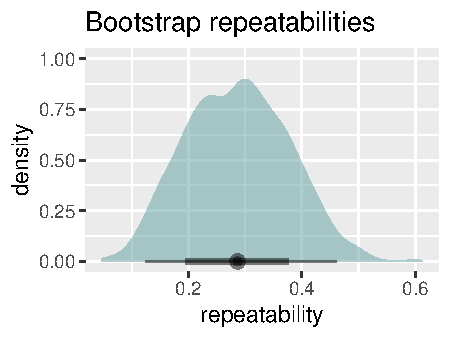
\includegraphics[width=0.4\linewidth]{RJ-2023-015_files/figure-latex/density-1} 

}

\caption{Density plot of the repeatabilities from the beetle model. The median bootstrap repeatability is approximatley .28 and denoted by a point under the density.  66\% and 95\% confidence intervals for the bootstrap repeatability are (0.217, 0.394) and (0.118, 0.475), respectively, and are displayed as line segments below the density.}\label{fig:density}
\end{figure}

\hypertarget{bootstrap-tests-for-a-single-parameter}{%
\subsubsection{Bootstrap tests for a single parameter}\label{bootstrap-tests-for-a-single-parameter}}

While \pkg{lmeresampler} was designed with a focus on estimation, the
bootstrap functions can be used to conduct bootstrap tests on individual parameters. For example, returning to the JSP example, we might be interested in generating approximate \(p\)-values for the fixed effects:

\begin{verbatim}
summary(jsp_mod)$coefficients
\end{verbatim}

\begin{verbatim}
#>                  Estimate Std. Error   t value
#> (Intercept)    14.1577509 0.73344165 19.303173
#> mathAge8        0.6388895 0.02544478 25.108865
#> genderM        -0.3571922 0.34009284 -1.050279
#> classnonmanual  0.7200815 0.38696812  1.860829
\end{verbatim}

To generate a bootstrap \(p\)-value for a fixed effect, we must generate \(B\) bootstrap resamples under the reduced model (i.e., the null hypothesis), refit the full model, and then calculate the \(t\)-statistic for each resample, denoted \(t^*_i\). The bootstrap \(p\)-value is then calculated as \((n_{\rm extreme} + 1) / (B + 1)\) (Davison and Hinkley 1997; Halekoh and Højsgaard 2014).

Using the \texttt{bootstrap()} function, you can implement this procedure for a single parameter. For example, if we wish to calculate the bootstrap \(p\)-value for the \texttt{class} fixed effect we first generate \(B=1000\) bootstrap samples from the reduced model without \texttt{class}. In this example, we use the Wild bootstrap to illustrate that we are not restricted to a parametric bootstrap.

\begin{verbatim}
reduced_model <- update(jsp_mod, . ~ . - class)
reduced_boot <- bootstrap(reduced_model, type = "wild", B = 1000, hccme = "hc2", 
                          aux.dist = "mammen", .refit = FALSE)
\end{verbatim}

\noindent Next, we refit the full model, \texttt{jsp\_mod}, to each simulation and extract the \(t\)-statistic for the \texttt{class} variable. Note that the function \texttt{extract\_t()} extracts the specified \(t\)-statistic from the coefficient table from model summary.

\begin{verbatim}
extract_t <- function(model, term) {
  coef(summary(model))[term, "t value"]
}

tstats <- purrr::map_dbl(
  reduced_boot, 
  ~refit(jsp_mod, .x) %>% extract_t(., term = "classnonmanual")
)
\end{verbatim}

\noindent With the bootstrap \(t\)-statistics in hand, we can approximate the \(p\)-value using basic logical and arithmetic operators

\begin{verbatim}
(sum(abs(tstats) >= extract_t(jsp_mod)) + 1) / (1000 + 1)
\end{verbatim}

\begin{verbatim}
#> [1] 0.2637363
\end{verbatim}

While the above process is not particularly difficult to implement using the tools provided by \pkg{lmeresampler}, things get tedious if multiple parameters are of interest in this summary table. To help reduce this burden on the user, we have provided the \texttt{bootstrap\_pvals()} function that will add bootstrap \(p\)-values for each term in the coefficient summary table. For \texttt{jsp\_mod}, this is achieved in the below code chunk:

\begin{verbatim}
bootstrap_pvals(jsp_mod, type = "wild", B = 1000, hccme = "hc2", aux.dist = "mammen")
\end{verbatim}

\begin{verbatim}
#> Bootstrap type: wild 
#> 
#> Number of resamples: 1000 
#> 
#> # A tibble: 4 x 5
#>   term           Estimate `Std. Error` `t value`  p.value
#>   <chr>             <dbl>        <dbl>     <dbl>    <dbl>
#> 1 (Intercept)      14.2         0.733      19.3  0.000999
#> 2 mathAge8          0.639       0.0254     25.1  0.000999
#> 3 genderM          -0.357       0.340      -1.05 0.257   
#> 4 classnonmanual    0.720       0.387       1.86 0.0569
\end{verbatim}

It's important to note that running bootstraps for each term in the model is computationally demanding. To speed up the computation, you can run the command in parallel, as we discuss below in \protect\hyperlink{bootstrapping-in-parallel}{Bootstrapping in parallel}.

\hypertarget{model-comparison}{%
\subsubsection{Model comparison}\label{model-comparison}}

The bootstrap can be useful during model selection.
For example, if you are comparing a full and reduced model where the reduced model has fewer random effects, a 50:50 mixture of \(\chi^2\) distributions is often used (Stram and Lee 1994); however, J. C. Pinheiro and Bates (2000) point out that this approximation is not always optimal. In this example, we explore the \texttt{Machine} data set discussed by J. C. Pinheiro and Bates (2000), which consists of productivity scores for six workers on three brands of machine. This data set can be loaded from \pkg{nlme}:

\begin{verbatim}
data("Machines", package = "nlme")
\end{verbatim}

J. C. Pinheiro and Bates (2000) consider two LME models for these data. The first model has a fixed effect for the machine and a random intercept for the worker.

\begin{verbatim}
reduced_mod <- lmer(score ~ Machine + (1 | Worker), data = Machines, REML = FALSE)
\end{verbatim}

The second model has the same fixed effects structure, but adds an additional random effect for the machine within the worker.

\begin{verbatim}
full_mod <- lmer(score ~ Machine + (1 | Worker/Machine), data = Machines, REML = FALSE)
\end{verbatim}

J. C. Pinheiro and Bates (2000) note that the approximate null distribution given by \(0.5\chi^2_0 + 0.5 \chi^2_1\) is not successful when the models are fit via maximum likelihood, and that the mixture is closer to \(0.65\chi^2_0 + 0.35 \chi^2_1\). Instead of relying on the conventional approximation, a bootstrap test can be conducted using \texttt{bootstrap()} to simulate the responses from the reduced model.

To conduct this bootstrap test, we first extract the observed statistic obtained via \texttt{anova()} and then generate \(B=1000\) bootstrap responses from the reduced model, \texttt{fm1\_machine}. Recall that specifying \texttt{.refit\ =\ FALSE} returns a data frame of the simulated responses. Here, we use a residual bootstrap for illustration.

\begin{verbatim}
observed <- anova(full_mod, reduced_mod)$Chisq[2]

reduced_boot <- bootstrap(reduced_mod, type = "residual", B = 1000, .refit = FALSE)
\end{verbatim}

Next, we must fit both the full and reduced models to the bootstrap responses and calculate the test statistic. The user-written \texttt{compare\_models()} function performs this refit and calculation for given models and bootstrap responses. The \texttt{control} argument for the full model was set to reduce the number of convergence warnings, since the null model had a variance component of 0 for machines within workers, so we expect warnings as we fit an expanded model.

\begin{verbatim}
compare_models <- function(full, reduced, newdata) {
  full_mod <- refit(full, newdata, 
                    control = lmerControl(check.conv.singular = "ignore", 
                                          check.conv.grad = "ignore"))
  reduced_mod <- refit(reduced, newdata)
  anova(full_mod, reduced_mod)$Chisq[2]
}
 
chisq_stats <- purrr::map_dbl(reduced_boot, ~compare_models(full_mod, reduced_mod, newdata = .x))
\end{verbatim}

With the test statistics in hand, we can quickly calculate the \(p\)-value

\begin{verbatim}
(sum(chisq_stats >= observed) + 1) / (1000 + 1)
\end{verbatim}

\begin{verbatim}
#> [1] 0.000999001
\end{verbatim}

\hypertarget{simulation-based-model-diagnostics}{%
\subsubsection{Simulation-based model diagnostics}\label{simulation-based-model-diagnostics}}

Our final example illustrates how the \texttt{bootstrap()} function can be used for model diagnosis. Loy, Hofmann, and Cook (2017) propose using the lineup protocol to diagnose LME models, since artificial structures often appear in conventional residual plots for this model class that are not indicative of a model deficiency.

In this example, we consider the \texttt{Dialyzer} data set provided by \pkg{nlme}. The data arise from a study characterizing the water transportation characteristics of 20 high flux membrane dialyzers, which were introduced to reduce the time a patient spends on hemodialysis (Vonesh and Carter 1992). The dialyzers were studied in vitro using bovine blood at flow rates of either 200 or 300 ml/min. The study measured the the ultrafiltration rate (ml/hr) at even transmembrane pressures (in mmHg). J. C. Pinheiro and Bates (2000) discuss modeling these data. Here, we explore how to create a lineup of residual plots to investigate the adequacy of the initial homoscedastic LME model fit by J. C. Pinheiro and Bates (2000).

\begin{verbatim}
library(nlme)
dialyzer_mod <- lme(
  rate ~ (pressure + I(pressure^2) + I(pressure^3) + I(pressure^4)) * QB, 
  data = Dialyzer, 
  random = ~ pressure + I(pressure^2)
)
\end{verbatim}

J. C. Pinheiro and Bates (2000) construct a residual plot of the conditional residuals plotted against the transmembrane pressure to explore the adequacy of the fitted model (Figure \ref{fig:residdialyzer}). There appears to be increasing spread of the conditional residuals, which would indicate that the homoscedastic model is not sufficient.

\begin{figure}

{\centering 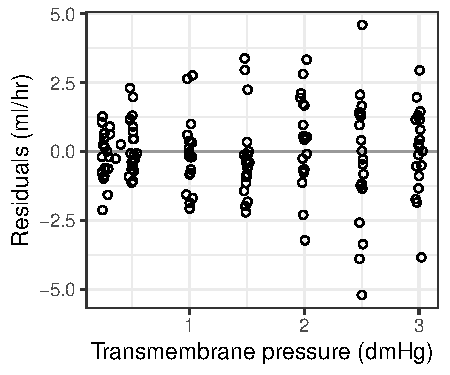
\includegraphics[width=0.4\linewidth]{RJ-2023-015_files/figure-latex/residdialyzer-1} 

}

\caption{A plot of the conditional residuals against the transmembrane pressure for the dialyzer model. It appears that the variability of the conditional residuals increases with transmembrance pressure, but does this indicate a model condition is violated?}\label{fig:residdialyzer}
\end{figure}

To check if this pattern is actually indicative of a problem, we construct a lineup of residual plots. To do this, we must generate data from a number of properly specified models, say 19, to serve as decoy residual plots. Then, we create a faceted set of residual plots where the observed residual plot (Figure \ref{fig:residdialyzer}) is randomly assigned to a facet. To generate the residuals from properly specified models, we use the parametric bootstrap via \texttt{bootstrap()} and extract a data frame containing the residuals from each bootstrap sample using \texttt{hlm\_resid()} from \CRANpkg{HLMdiag} (Loy and Hofmann 2014).

\begin{verbatim}
set.seed(1234)
library(HLMdiag)
sim_resids <- bootstrap(dialyzer_mod, .f = hlm_resid, type = "parametric", B = 19)
\end{verbatim}

\noindent The simulated residuals are stored in the \texttt{replicates} element of the \texttt{sim\_resids} list. \texttt{sim\_resids\$replicates} is a tibble containing the 19 bootstrap samples, with the the replicate number stored in the \texttt{.n} column.

\begin{verbatim}
dplyr::glimpse(sim_resids$replicates)
\end{verbatim}

\begin{verbatim}
#> Rows: 2,660
#> Columns: 15
#> $ id              <dbl> 1, 2, 3, 4, 5, 6, 7, 8, 9, 10, 11, 12, 13, 14, 15, 16,~
#> $ rate            <dbl> -0.8579226, 17.0489029, 34.3658738, 44.8495547, 44.525~
#> $ pressure        <dbl> 0.240, 0.505, 0.995, 1.485, 2.020, 2.495, 2.970, 0.240~
#> $ `I(pressure^2)` <I<dbl>>   0.0576, 0.255025, 0.990025, 2.205225,   4.0804, 6~
#> $ `I(pressure^3)` <I<dbl>>     0.013824,  0.128787625,  0.985074875,  3.274759~
#> $ `I(pressure^4)` <I<dbl>>   0.00331776, 0.065037...., 0.980149...., 4.863017.~
#> $ QB              <fct> 200, 200, 200, 200, 200, 200, 200, 200, 200, 200, 200,~
#> $ Subject         <ord> 1, 1, 1, 1, 1, 1, 1, 2, 2, 2, 2, 2, 2, 2, 3, 3, 3, 3, ~
#> $ .resid          <dbl> -1.19758632, 0.65600425, -0.90104247, 1.39131045, 0.11~
#> $ .fitted         <dbl> 0.3396637, 16.3928987, 35.2669162, 43.4582443, 44.4100~
#> $ .ls.resid       <dbl> -0.51757746, 1.23968783, -1.32231163, 0.59071041, 0.30~
#> $ .ls.fitted      <dbl> -0.3403452, 15.8092151, 35.6881854, 44.2588443, 44.223~
#> $ .mar.resid      <dbl> -2.1236410, -0.3100360, -2.1298323, -0.3453118, -2.455~
#> $ .mar.fitted     <dbl> 1.265718, 17.358939, 36.495706, 45.194867, 46.981057, ~
#> $ .n              <int> 1, 1, 1, 1, 1, 1, 1, 1, 1, 1, 1, 1, 1, 1, 1, 1, 1, 1, ~
\end{verbatim}

Now, we use the \texttt{lineup()} function from \CRANpkg{nullabor} (Buja et al. 2009) to generate the lineup data. \texttt{lineup()} will randomly insert the observed (\texttt{true}) data into the \texttt{samples} data, ``encrypt'' the position of the observed data, and print a message that you can later decrypt in the console.

\begin{verbatim}
library(nullabor)
lineup_data <- lineup(true = hlm_resid(dialyzer_mod), n = 19, samples = sim_resids$replicates)
\end{verbatim}

\begin{verbatim}
#> decrypt("CLg7 X161 sO bJws6sJO qj")
\end{verbatim}

\begin{verbatim}
dplyr::glimpse(lineup_data)
\end{verbatim}

\begin{verbatim}
#> Rows: 2,800
#> Columns: 15
#> $ id              <dbl> 1, 2, 3, 4, 5, 6, 7, 8, 9, 10, 11, 12, 13, 14, 15, 16,~
#> $ rate            <dbl> -0.8579226, 17.0489029, 34.3658738, 44.8495547, 44.525~
#> $ pressure        <dbl> 0.240, 0.505, 0.995, 1.485, 2.020, 2.495, 2.970, 0.240~
#> $ `I(pressure^2)` <I<dbl>>   0.0576, 0.255025, 0.990025, 2.205225,   4.0804, 6~
#> $ `I(pressure^3)` <I<dbl>>     0.013824,  0.128787625,  0.985074875,  3.274759~
#> $ `I(pressure^4)` <I<dbl>>   0.00331776, 0.065037...., 0.980149...., 4.863017.~
#> $ QB              <fct> 200, 200, 200, 200, 200, 200, 200, 200, 200, 200, 200,~
#> $ Subject         <ord> 1, 1, 1, 1, 1, 1, 1, 2, 2, 2, 2, 2, 2, 2, 3, 3, 3, 3, ~
#> $ .resid          <dbl> -1.19758632, 0.65600425, -0.90104247, 1.39131045, 0.11~
#> $ .fitted         <dbl> 0.3396637, 16.3928987, 35.2669162, 43.4582443, 44.4100~
#> $ .ls.resid       <dbl> -0.51757746, 1.23968783, -1.32231163, 0.59071041, 0.30~
#> $ .ls.fitted      <dbl> -0.3403452, 15.8092151, 35.6881854, 44.2588443, 44.223~
#> $ .mar.resid      <dbl> -2.1236410, -0.3100360, -2.1298323, -0.3453118, -2.455~
#> $ .mar.fitted     <dbl> 1.265718, 17.358939, 36.495706, 45.194867, 46.981057, ~
#> $ .sample         <dbl> 1, 1, 1, 1, 1, 1, 1, 1, 1, 1, 1, 1, 1, 1, 1, 1, 1, 1, ~
\end{verbatim}

\noindent With the lineup data in hand, we can create a lineup of residual plots using \texttt{facet\_wrap()}:

\begin{verbatim}
ggplot(lineup_data, aes(x = pressure, y = .resid)) +
  geom_hline(yintercept = 0, color = "gray60") +
  geom_point(shape = 1) +
  facet_wrap(~.sample) +
  theme_bw() +
  labs(x = "Transmembrane pressure (dmHg)", y = "Residuals (ml/hr)")
\end{verbatim}

\begin{figure}

{\centering 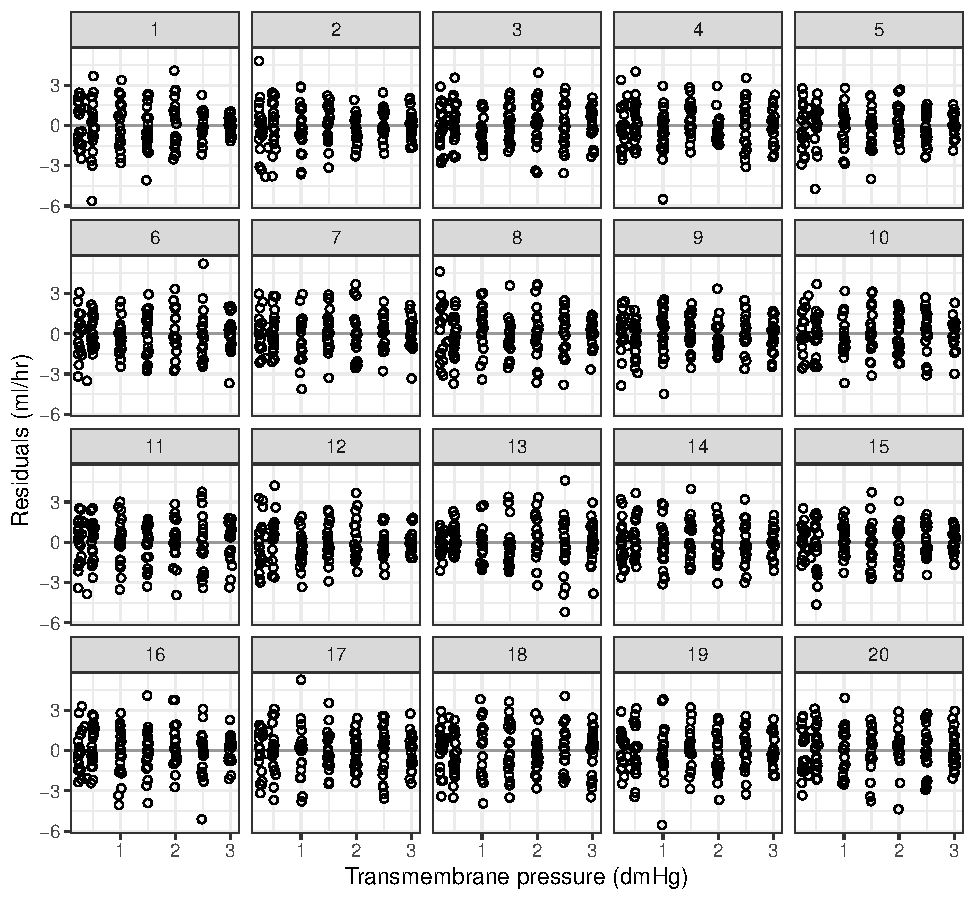
\includegraphics{RJ-2023-015_files/figure-latex/lineup-1} 

}

\caption{A lineup of the conditional residuals against the transmembrane pressure for the dialyzer model. One of the facets contains the true residual plot generated from the fitted model, the others are decoys generated using a parametric bootstrap. Facet 13 contains the observed residuals and is discernibly different from decoy plots, providing evidence of that a model condition has been violated.}\label{fig:lineup}
\end{figure}

\noindent In Figure \ref{fig:lineup}, the observed residual plot is in position 13. If you can discern this plot from the field of decoys, then there is evidence that the fitted homogeneous LME model is deficient. In this case, we believe 13 is discernibly different, as expected based on the discussion in J. C. Pinheiro and Bates (2000).

Since we have discovered signs of within-group heteroscedasticity, we could reformulate our model via \texttt{nlme::lme()} adding a \texttt{weights} argument using \texttt{varPower}, or we could utilize the Wild bootstrap, as illustrated below.

\begin{verbatim}
wild_dialyzer <- bootstrap(dialyzer_mod, .f = fixef, type = "wild", B = 1000, 
                           hccme = "hc2", aux.dist = "webb")

confint(wild_dialyzer, type = "perc")
\end{verbatim}

\begin{verbatim}
#> # A tibble: 10 x 6
#>    term                estimate  lower   upper type  level
#>    <chr>                  <dbl>  <dbl>   <dbl> <chr> <dbl>
#>  1 (Intercept)          -16.0   -18.0  -13.9   perc   0.95
#>  2 pressure              88.4    77.4   99.1   perc   0.95
#>  3 I(pressure^2)        -44.3   -57.1  -30.8   perc   0.95
#>  4 I(pressure^3)          9.17    2.45  15.5   perc   0.95
#>  5 I(pressure^4)         -0.690  -1.70   0.425 perc   0.95
#>  6 QB300                 -1.26   -4.55   2.06  perc   0.95
#>  7 pressure:QB300         0.621 -16.0   16.9   perc   0.95
#>  8 I(pressure^2):QB300    3.15  -18.5   27.6   perc   0.95
#>  9 I(pressure^3):QB300    0.102 -12.0   11.1   perc   0.95
#> 10 I(pressure^4):QB300   -0.172  -1.98   1.84  perc   0.95
\end{verbatim}

\hypertarget{bootstrapping-in-parallel}{%
\subsection{Bootstrapping in parallel}\label{bootstrapping-in-parallel}}

Bootstrapping is a computationally demanding task, but bootstrap iterations do not rely on each other so they are easy to implement in parallel. Rather than building parallel processing into \pkg{lmeresampler}, we created a utility function, \texttt{combine\_lmeresamp()}, that allows the user to easily implement parallel processing using \pkg{doParallel} (Microsoft and Weston 2020a) and \pkg{foreach} (Microsoft and Weston 2020b). The code is thus concise and simple enough for users without much experience with parallelization, while also providing flexibility to the user.

\CRANpkg{doParallel} and \CRANpkg{foreach} default to multicore (i.e., forking) functionality when using parallel computing on UNIX operating systems and snow-like (i.e., clustering) functionality on Windows systems. In this section, we will use clustering in our example. For more information on forking, we refer the reader to the vignette in Microsoft and Weston (2020a).

The basic idea behind clustering is to execute tasks as a ``cluster'' of computers. Each cluster needs to be fed in information separately, and as a consequence clustering has more overhead than forking. Clusters also need to be made and stopped with each call to \texttt{foreach()} to explicitly tell the CPU when to begin and end the parallelization.

Below, we revisit the JSP example and distribute 2000 bootstrap iterations equally over two cores:

\begin{verbatim}
library(foreach)
library(doParallel)
\end{verbatim}

\begin{verbatim}
#> Loading required package: iterators
\end{verbatim}

\begin{verbatim}
#> Loading required package: parallel
\end{verbatim}

\begin{verbatim}
set.seed(5678)

# Starting a cluster with 2 cores
no_cores <- 2
cl <- makeCluster(no_cores)
registerDoParallel(cores = no_cores)

# Run 1000 bootstrap iterations on each core
boot_parallel <- foreach(
  B = rep(1000, 2), 
  .combine = combine_lmeresamp,
  .packages = c("lmeresampler", "lme4")
) %dopar% {
  bootstrap(jsp_mod, .f = fixef, type = "parametric", B = B)
}

# Stop the cluster
stopCluster(cl)
\end{verbatim}

\noindent The \texttt{combine\_lmeresamp()} function combines the two \texttt{lmeresamp} objects that are returned from the two \texttt{bootstrap()} calls into a single \texttt{lmeresamp} object. Consequently, working with the returned object proceeds as previously discussed.

It's important to note that running a process on two cores does not yield a runtime that is twice as fast as running the same process on one core. This is because parallelization takes some overhead to split the processes, so while runtime will substantially improve, it will not correspond exactly to the number of cores being used. For example, the runtime for the JSP example run on a single core was

\begin{verbatim}
#>    user  system elapsed 
#>  23.084   1.212  24.376
\end{verbatim}

\noindent and the runtime for the JSP run on two cores was

\begin{verbatim}
#>    user  system elapsed 
#>  23.550   1.800  12.747
\end{verbatim}

\noindent These timings were generated using \texttt{system.time()} on a MacBook Pro with a 2.9 GHz Quad-Core Intel Core i7 processor. In this set up, running the 2000 bootstrap iterations over two cores reduced the runtime by a factor of about 1.91, but this will vary based on the hardware and setting used.

\hypertarget{summary}{%
\subsection{Summary}\label{summary}}

In this paper, we discussed our implementation of five bootstrap procedures for nested, Gaussian-response LME models fit via the \pkg{nlme} or \pkg{lme4} packages. The \code{bootstrap()} function in \pkg{lmeresampler} provides a unified interface to these procedures, allowing users to easily bootstrap their fitted LME models. In our examples, we illustrated the basic usage of the bootstrap, how it can be used to estimate functions of parameters, how it can be used for testing, and how it can be used to create simulation-based visual diagnostics. The bootstrap approach to inference is computationally intensive, so we have also demonstrated how users can bootstrap in parallel.

While this paper focused solely on the nested, Gaussian-response LME model, \pkg{lmeresampler} implements bootstrap procedures for a wide class of models. Specifically, the cases, residual, and parametric bootstraps can be used to bootstrap generalized LME models fit via \code{lme4::glmer()}. Additionally, the parametric bootstrap works with LME models with crossed random effects, though the results may not be optimal (Mccullagh 2000). Future development of \pkg{lmeresampler} will focus on implementing additional extensions, especially for crossed data structures.

\hypertarget{acknowledgements}{%
\subsection{Acknowledgements}\label{acknowledgements}}

We thank Spenser Steele for his contributions to the original code base of \pkg{lmeresampler}. We also thank the reviewers and associate editor whose comments improved the quality of this paper.

\hypertarget{references}{%
\section*{References}\label{references}}
\addcontentsline{toc}{section}{References}

\hypertarget{refs}{}
\begin{CSLReferences}{1}{0}
\leavevmode\vadjust pre{\hypertarget{ref-lme4}{}}%
Bates, Douglas, Martin Mächler, Ben Bolker, and Steve Walker. 2015. {``Fitting Linear Mixed-Effects Models Using {lme4}.''} \emph{Journal of Statistical Software} 67 (1): 1--48. \url{https://doi.org/10.18637/jss.v067.i01}.

\leavevmode\vadjust pre{\hypertarget{ref-buja2009}{}}%
Buja, Andreas, Dianne Cook, Heike Hofmann, Michael Lawrence, Eun-kyung Lee, Deborah F. Swayne, and Hadley Wickham. 2009. {``Statistical Inference for Exploratory Data Analysis and Model Diagnostics.''} \emph{Royal Society Philosophical Transactions A} 367 (1906): 4361--83. \url{https://doi.org/10.1098/rsta.2009.0120}.

\leavevmode\vadjust pre{\hypertarget{ref-Carpenter:2003uy}{}}%
Carpenter, James R, Harvey Goldstein, and Jon Rasbash. 2003. {``A Novel Bootstrap Procedure for Assessing the Relationship Between Class Size and Achievement.''} \emph{Journal of the Royal Statistical Society, Series C} 52 (4): 431--43. \url{https://doi.org/10.1111/1467-9876.00415}.

\leavevmode\vadjust pre{\hypertarget{ref-Chambers:2013ba}{}}%
Chambers, Raymond, and Hukum Chandra. 2013. {``A Random Effect Block Bootstrap for Clustered Data.''} \emph{Journal of Computational and Graphical Statistics} 22 (2): 452--70. \url{https://doi.org/10.1080/10618600.2012.681216}.

\leavevmode\vadjust pre{\hypertarget{ref-Davidson2008-vq}{}}%
Davidson, Russell, and Emmanuel Flachaire. 2008. {``The Wild Bootstrap, Tamed at Last.''} \emph{Journal of Econometrics} 146 (1): 162--69. \url{https://doi.org/10.1016/j.jeconom.2008.08.003}.

\leavevmode\vadjust pre{\hypertarget{ref-davison-hinkley}{}}%
Davison, A. C., and D. V. Hinkley. 1997. \emph{Boostrap Methods and Their Application}. Cambridge University Press.

\leavevmode\vadjust pre{\hypertarget{ref-clme}{}}%
Farnan, Laura, Anastasia Ivanova, and Shyamal D. Peddada. 2014. {``Linear Mixed Efects Models Under Inequality Constraints with Applications.''} \emph{PLOS ONE} 9 (1). \url{https://doi.org/10.1371/journal.pone.0084778}.

\leavevmode\vadjust pre{\hypertarget{ref-Field:2007vm}{}}%
Field, Christopher A, and A H Welsh. 2007. {``Bootstrapping Clustered Data.''} \emph{Journal of the Royal Statistical Society, Series B} 69 (3): 369--90. \url{https://doi.org/10.1111/j.1467-9868.2007.00593.x}.

\leavevmode\vadjust pre{\hypertarget{ref-Flachaire2005-qo}{}}%
Flachaire, Emmanuel. 2005. {``Bootstrapping Heteroskedastic Regression Models: Wild Bootstrap Vs. Pairs Bootstrap.''} \emph{Computational Statistics \& Data Analysis} 49 (2): 361--76. \url{https://doi.org/10.1016/j.csda.2004.05.018}.

\leavevmode\vadjust pre{\hypertarget{ref-galecki2013}{}}%
Galecki, Andrzej, and Tomasz Burzykowski. 2013. \emph{Linear Mixed-Effects Models Using r: A Step-by-Step Approach}. New York: Springer. \url{https://doi.org/10.1007/978-1-4614-3900-4}.

\leavevmode\vadjust pre{\hypertarget{ref-goldstein2011}{}}%
Goldstein, Harvey. 2011. \emph{Multilevel Statistical Models}. 4th ed. West Sussex: John Wiley \& Sons, Ltd. \url{https://doi.org/10.1002/9780470973394}.

\leavevmode\vadjust pre{\hypertarget{ref-pbkrtest}{}}%
Halekoh, Ulrich, and Søren Højsgaard. 2014. {``A Kenward-Roger Approximation and Parametric Bootstrap Methods for Tests in Linear Mixed Models -- the {R} Package {pbkrtest}.''} \emph{Journal of Statistical Software} 59 (9): 1--30. \url{https://doi.org/10.18637/jss.v059.i09}.

\leavevmode\vadjust pre{\hypertarget{ref-Haslett2007-kl}{}}%
Haslett, John, and Stephen J Haslett. 2007. {``The Three Basic Types of Residuals for a Linear Model.''} \emph{International Statistical Review} 75 (1): 1--24. \url{https://doi.org/10.1111/j.1751-5823.2006.00001.x}.

\leavevmode\vadjust pre{\hypertarget{ref-Hui2021-cx}{}}%
Hui, Francis K C, Samuel Müller, and Alan H Welsh. 2021. {``Random Effects Misspecification Can Have Severe Consequences for Random Effects Inference in Linear Mixed Models.''} \emph{International Statistical Review = Revue Internationale de Statistique} 89 (1): 186--206. \url{https://doi.org/10.1111/insr.12378}.

\leavevmode\vadjust pre{\hypertarget{ref-Jacqmin-Gadda2007-ll}{}}%
Jacqmin-Gadda, Hélène, Solenne Sibillot, Cécile Proust, Jean-Michel Molina, and Rodolphe Thiébaut. 2007. {``Robustness of the Linear Mixed Model to Misspecified Error Distribution.''} \emph{Computational Statistics \& Data Analysis} 51 (10): 5142--54. \url{https://doi.org/10.1016/j.csda.2006.05.021}.

\leavevmode\vadjust pre{\hypertarget{ref-ggdist}{}}%
Kay, Matthew. 2021. \emph{{ggdist}: Visualizations of Distributions and Uncertainty}. \url{https://doi.org/10.5281/zenodo.3879620}.

\leavevmode\vadjust pre{\hypertarget{ref-Liu1988-zw}{}}%
Liu, Regina Y. 1988. {``Bootstrap Procedures Under Some Non-i.i.d. Models.''} \emph{Annals of Statistics} 16 (4): 1696--1708. \url{https://doi.org/10.1214/aos/1176351062}.

\leavevmode\vadjust pre{\hypertarget{ref-hlmdiag}{}}%
Loy, Adam, and Heike Hofmann. 2014. {``{HLMdiag}: A Suite of Diagnostics for Hierarchical Linear Models in {R}.''} \emph{Journal of Statistical Software} 56 (5): 1--28. \url{https://doi.org/10.18637/jss.v056.i05}.

\leavevmode\vadjust pre{\hypertarget{ref-Loy2017-fo}{}}%
Loy, Adam, Heike Hofmann, and Dianne Cook. 2017. {``Model Choice and Diagnostics for Linear {Mixed-Effects} Models Using Statistics on Street Corners.''} \emph{Journal of Computational and Graphical Statistics} 26 (3): 478--92. \url{https://doi.org/10.1080/10618600.2017.1330207}.

\leavevmode\vadjust pre{\hypertarget{ref-Mammen1993-eo}{}}%
Mammen, Enno. 1993. {``Bootstrap and Wild Bootstrap for High Dimensional Linear Models.''} \emph{Annals of Statistics} 21 (1): 255--85. \url{https://doi.org/10.1214/aos/1176349025}.

\leavevmode\vadjust pre{\hypertarget{ref-Mccullagh2000-st}{}}%
Mccullagh, Peter. 2000. {``Resampling and Exchangeable Arrays.''} \emph{Bernoulli} 6 (2): 285--301. \url{https://doi.org/10.2307/3318577}.

\leavevmode\vadjust pre{\hypertarget{ref-doparallel}{}}%
Microsoft, and Steve Weston. 2020a. \emph{doParallel: Foreach Parallel Adaptor for the 'Parallel' Package}. \url{https://CRAN.R-project.org/package=doParallel}.

\leavevmode\vadjust pre{\hypertarget{ref-foreach}{}}%
Microsoft, and Steve Weston. 2020b. \emph{Foreach: Provides Foreach Looping Construct}. \url{https://CRAN.R-project.org/package=foreach}.

\leavevmode\vadjust pre{\hypertarget{ref-Modugno2015-kd}{}}%
Modugno, Lucia, and Simone Giannerini. 2015. {``The Wild Bootstrap for Multilevel Models.''} \emph{Communications in Statistics - Theory and Methods} 44 (22): 4812--25. \url{https://doi.org/10.1080/03610926.2013.802807}.

\leavevmode\vadjust pre{\hypertarget{ref-Morris:2002tj}{}}%
Morris, Jeffrey S. 2002. {``{The BLUPs are not {``}best{''} when it comes to bootstrapping}.''} \emph{Statistics and Probability Letters} 56 (4): 425--30. \url{https://doi.org/10.1016/S0167-7152(02)00041-X}.

\leavevmode\vadjust pre{\hypertarget{ref-Mortimore1988-xv}{}}%
Mortimore, Peter, Pamela Sammons, Louise Stoll, and Russell Ecob. 1988. \emph{School Matters}. University of California Press.

\leavevmode\vadjust pre{\hypertarget{ref-Nakagawa2010-co}{}}%
Nakagawa, Shinichi, and Holger Schielzeth. 2010. {``Repeatability for Gaussian and Non-Gaussian Data: A Practical Guide for Biologists.''} \emph{Biological Reviews of the Cambridge Philosophical Society} 85 (4): 935--56. \url{https://doi.org/10.1111/j.1469-185X.2010.00141.x}.

\leavevmode\vadjust pre{\hypertarget{ref-Pinhiero:2000vf}{}}%
Pinheiro, Jose C, and Douglas M Bates. 2000. \emph{Mixed-Effects Models in s and s-PLUS}. New York: Springer-Verlag. \url{https://doi.org/10.1007/b98882}.

\leavevmode\vadjust pre{\hypertarget{ref-nlme}{}}%
Pinheiro, Jose, Douglas Bates, Saikat DebRoy, Deepayan Sarkar, and R Core Team. 2017. \emph{{nlme}: Linear and Nonlinear Mixed Effects Models}. \url{https://CRAN.R-project.org/package=nlme}.

\leavevmode\vadjust pre{\hypertarget{ref-raudenbush}{}}%
Raudenbush, Stephen W., and Anthony S. Bryk. 2002. \emph{Hierarchical Linear Models: Applications and Data Analysis Methods}. 2nd ed. Thousand Oaks, CA: Sage Publications, Inc.

\leavevmode\vadjust pre{\hypertarget{ref-Sanchez-Espigares2009-yg}{}}%
Sánchez-Espigares, José A, and Jordi Ocaña. 2009. {``An {R} Implementation of Bootstrap Procedures for Mixed Models.''} Rennes, France: The R User Conference 2009. \url{https://www.r-project.org/conferences/useR-2009/slides/SanchezEspigares+Ocana.pdf}.

\leavevmode\vadjust pre{\hypertarget{ref-rlrsim}{}}%
Scheipl, Fabian, Sonja Greven, and Helmut Kuechenhoff. 2008. {``Size and Power of Tests for a Zero Random Effect Variance or Polynomial Regression in Additive and Linear Mixed Models.''} \emph{Computational Statistics \& Data Analysis} 52 (7): 3283--99. \url{https://doi.org/10.1016/j.csda.2007.10.022}.

\leavevmode\vadjust pre{\hypertarget{ref-shao1995jackknife}{}}%
Shao, Jun, and Dongsheng Tu. 1995. \emph{The Jackknife and Bootstrap}. Springer.

\leavevmode\vadjust pre{\hypertarget{ref-Singer2017-sd}{}}%
Singer, Julio M, Francisco M M Rocha, and Juvêncio S Nobre. 2017. {``Graphical Tools for Detecting Departures from Linear Mixed Model Assumptions and Some Remedial Measures.''} \emph{International Statistical Review = Revue Internationale de Statistique} 85 (2): 290--324. \url{https://doi.org/10.1111/insr.12178}.

\leavevmode\vadjust pre{\hypertarget{ref-rptR}{}}%
Stoffel, Martin A., Shinichi Nakagawa, and Holger Schielzeth. 2017. {``{rptR}: Repeatability Estimation and Variance Decomposition by Generalized Linear Mixed-Effects Models.''} \emph{Methods in Ecology and Evolution} 8: 1639--44. \url{https://doi.org/10.1111/2041-210X.12797}.

\leavevmode\vadjust pre{\hypertarget{ref-Stram:1994wd}{}}%
Stram, Daniel O, and Jae Won Lee. 1994. {``Variance Components Testing in the Longitudinal Mixed Effects Model.''} \emph{Biometrics} 50 (4): 1171--77.

\leavevmode\vadjust pre{\hypertarget{ref-VanderLeeden:2008}{}}%
Van der Leeden, Rien, Erik Meijer, and Frank M. T. A. Busing. 2008. {``Resampling Multilevel Models.''} In \emph{Handbook of Multilevel Analysis}, edited by Jan de Leeuw and Erik Meijer, 401--33. Springer New York. \url{https://doi.org/10.1007/978-0-387-73186-5_11}.

\leavevmode\vadjust pre{\hypertarget{ref-Vonesh:1992us}{}}%
Vonesh, Edward F, and Randy L Carter. 1992. {``Mixed-Effects Nonlinear Regression for Unbalanced Repeated Measures.''} \emph{Biometrics} 48 (1): 1--17.

\leavevmode\vadjust pre{\hypertarget{ref-Webb2013-nw}{}}%
Webb, Matthew D. 2013. {``Reworking Wild Bootstrap Based Inference for Clustered Errors.''} Queen's Economics Department Working Paper. \url{https://www.econstor.eu/handle/10419/97480}.

\end{CSLReferences}

\bibliography{loy.bib}

\address{%
Adam Loy\\
Carleton College\\%
Northfield, MN, USA\\
%
\url{https://aloy.rbind.io/}\\%
\textit{ORCiD: \href{https://orcid.org/0000-0002-5780-4611}{0000-0002-5780-4611}}\\%
\href{mailto:aloy@carleton.edu}{\nolinkurl{aloy@carleton.edu}}%
}

\address{%
Jenna Korobova\\
Carleton College\\%
Northfield, MN, USA\\
%
%
%
\href{mailto:jenna.korobova@gmail.com}{\nolinkurl{jenna.korobova@gmail.com}}%
}
